\documentclass{weekly}
\begin{document}
\maketitlew{Аналитическая механика}{1}{6}{23}

\begin{wrapfigure}{r}{.28\textwidth}
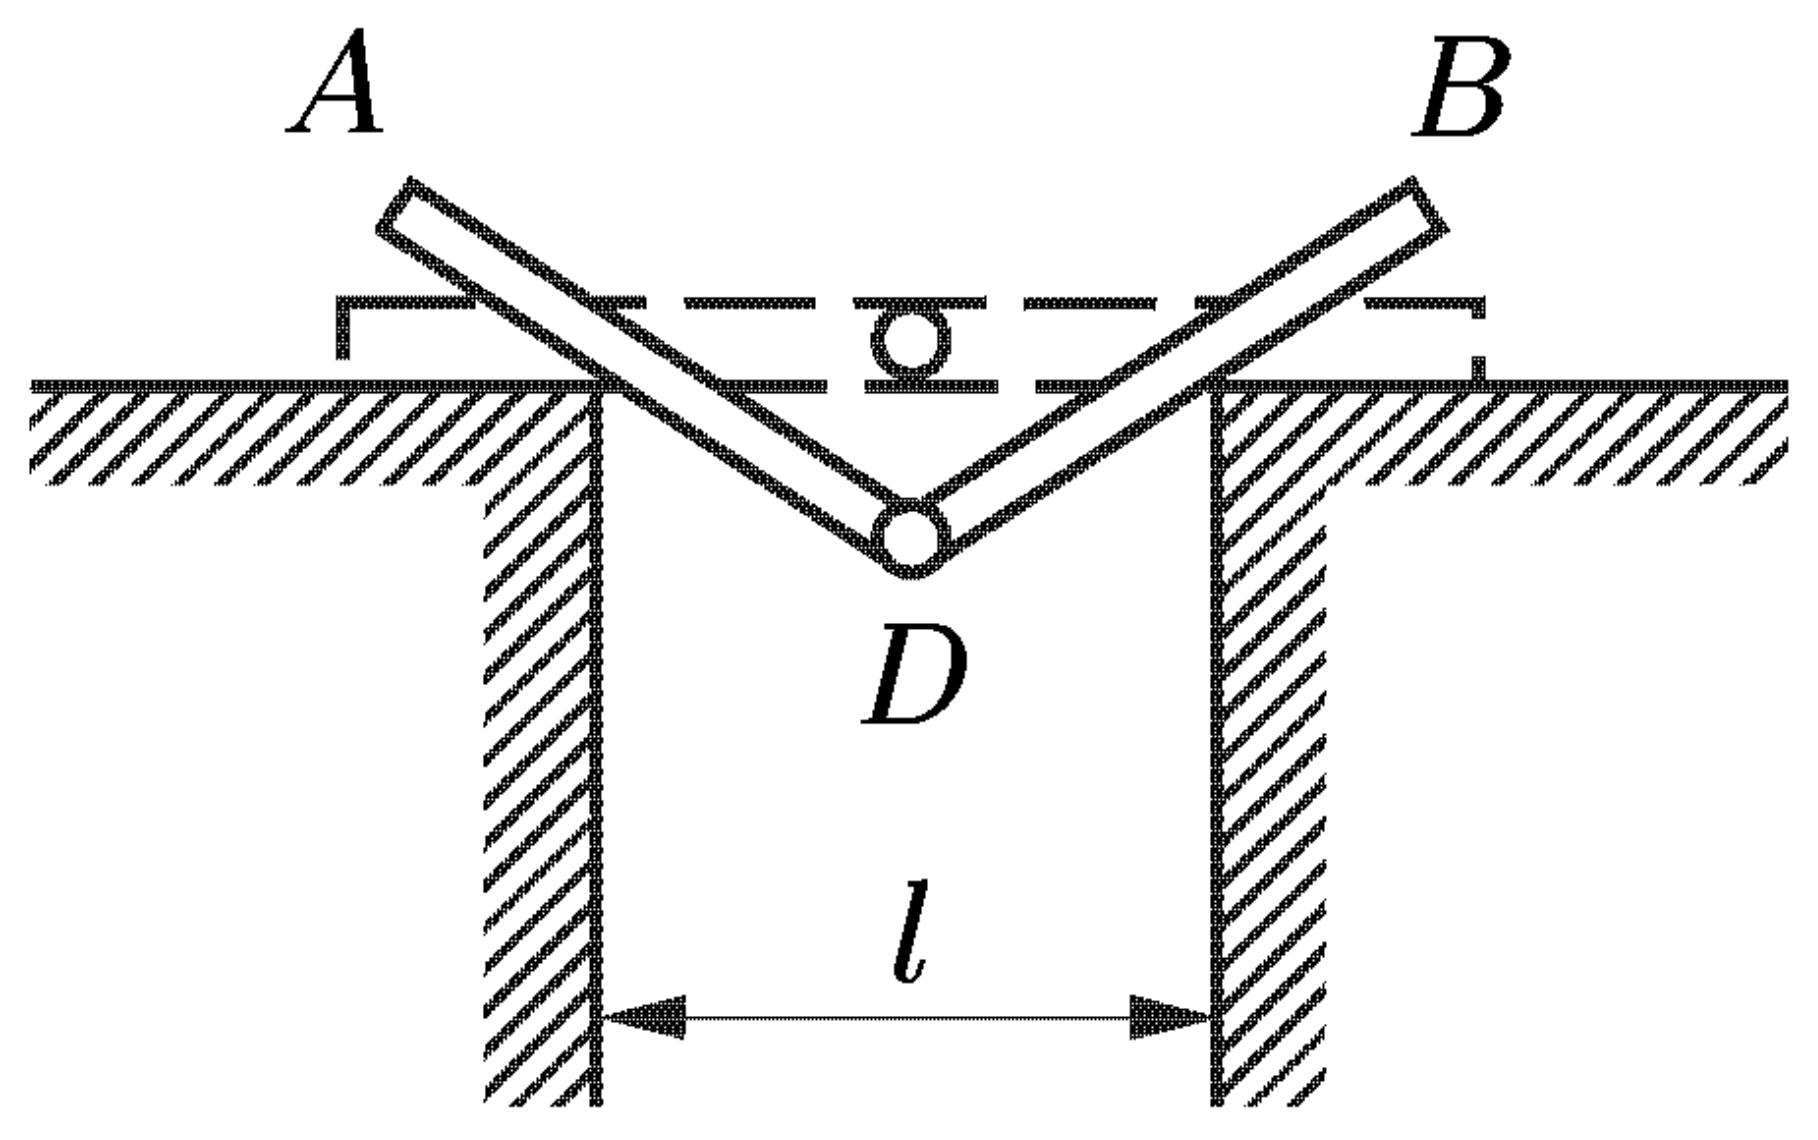
\includegraphics[width=\linewidth]{7-29}
\end{wrapfigure}
\paragraph{7.29.} Однородные стержни~$AD$ и~$BD$, шарнирно соединённые
в~точке~$D$, опираются на~два гладких угла. Длина каждого стержня
равна расстоянию между опорами~$l$. В~начальный момент стержни
горизонтальны и~расположены симметрично относительно опор,
а~затем (после малого начального толчка) приходят в~движение
за~счёт собственного веса, причём точка~$D$ перемещается по~вертикали.
Определить скорость точки~$D$ в~момент, когда концы стержней~$A$ и~$B$
достигнут угловых точек.

$\blacktriangleright$ При~решении задачи~3.12 было показано,
что~скорость~$v_T$ точки касания стержня вершины угла
направлена вдоль стержня и~связана со~скоростью точки~$D$
и~углом между стержнями~$\varphi$ соотношением
\begin{equation}
    v_T = v_D \cos\frac\varphi 2.
\end{equation}

Применив закон сохранения энергии и~теорему Кёнига, получим
для~рассматриваемого момента времени ($\varphi\to\varphi_0 = 60^\circ$):
\begin{equation}
    0 = -2 \cdot g\frac{l \cos\frac{\varphi_0}{2}}{2} +
            2 \cdot \frac{v_C^2}{2} +
            2 \cdot \frac{l^2}{12} \frac{\omega^2}{2}.
    \label{7.29:energy}
\end{equation}

$\triangleright$ Пусть концы~$\vec r_1$ и~$\vec r_2$ однородного стержня,
совершающего плоскопараллельное движение, имеют скорости~$\vec v_1$
и~$\vec v_2$. Найдём скорость~$\vec v_C$ его центра масс
и~угловую скорость~$\omega$:
\begin{align}
    \vec r_C = \dfrac{\vec r_1 + \vec r_2}{2}
&\then
    \vec v_C = \dfrac{\vec v_1 + \vec v_2}{2};
\\
    \vec v_2 - \vec v_1 = \vec\omega \times (\vec r_2 - \vec r_1)
&\then
    \vec\omega \times (\vec v_2 - \vec v_1)
        = -\omega^2 (\vec r_2 - \vec r_1).
\end{align}
Последнее соотношение скаляризируем как
\begin{equation}
    \omega = \frac{\abs{v_2^{\perp} - v_1^{\perp}}}{l},
\end{equation}
что, в~общем-то, и~так было понятно. \hfill $\triangleleft$

Выполним соответствующие подстановки в~\eqref{7.29:energy}:
\begin{gather}
    \frac{\sqrt{3}}{2} gl = v_C^2 + \frac{1}{3} \omega^2 l^2
        = \left(v_T^2 + \frac{1}{4} \omega^2 l^2\right)
            + \frac{1}{12} \omega^2 l^2
        = v_D^2 \left(\cos^2\frac{\varphi_0}{2}
            + \frac{1}{3} \sin^2\frac{\varphi_0}{2}\right).
\end{gather}
\textbf{Ответ:}\qquad $v_D = \sqrt{\dfrac{3\sqrt{3}}{5}}$.
\hfill $\blacktriangleleft$

\bigskip
\begin{small}
\textsl{Примечание.} Вообще говоря, стержни оторвутся от~углов
раньше рассматриваемого момента времени.
Доказывать это утверждение здесь и~сейчас я, конечно же, не~буду.
\end{small}


\begin{wrapfigure}[6]{r}{.42\textwidth}
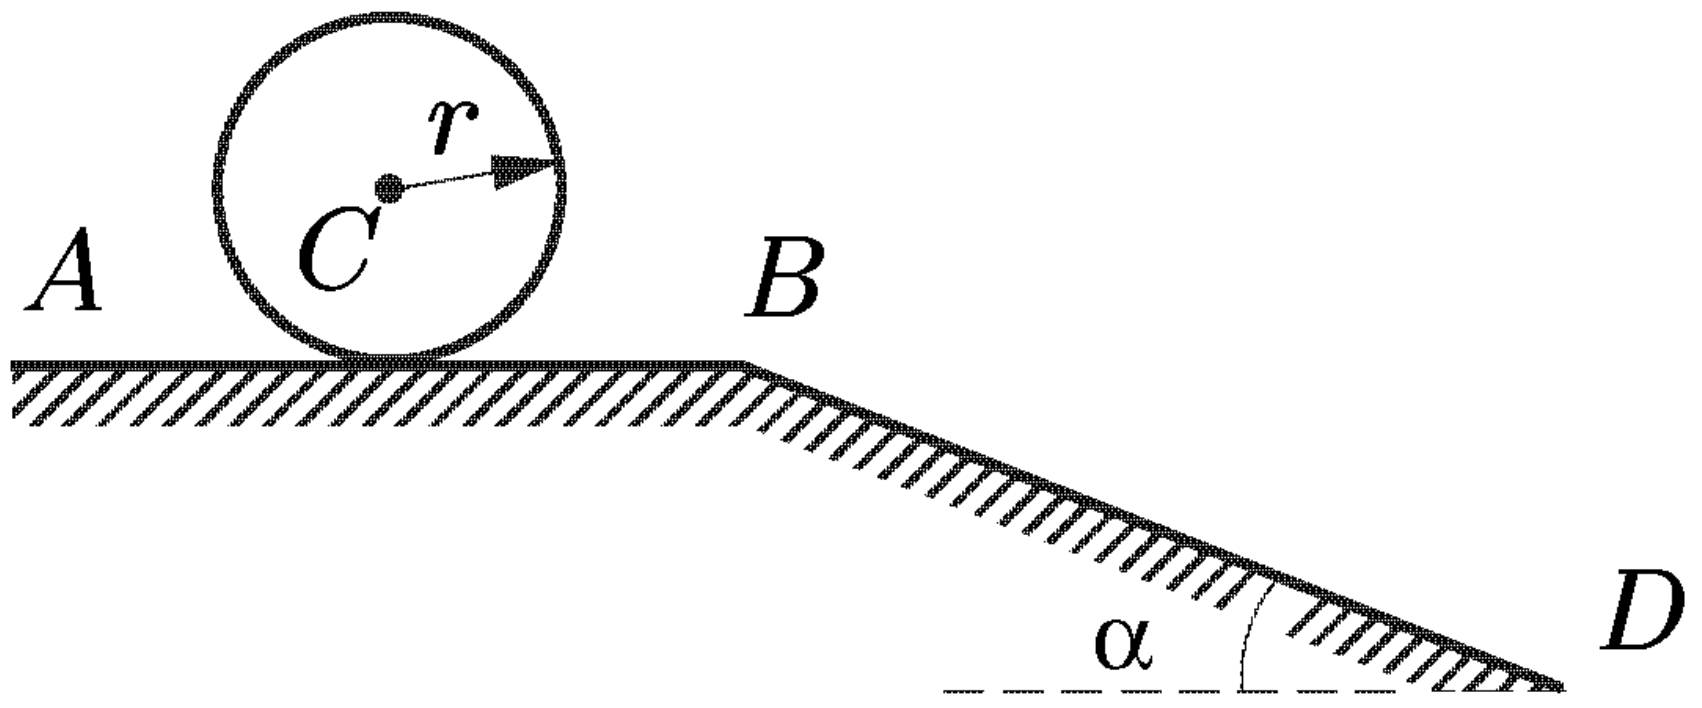
\includegraphics[width=\linewidth]{7-42}
\end{wrapfigure}
\paragraph{7.42.} Шар радиуса~$r$ катится без~проскальзывания
по~горизонтальной плоскости~$AB$, переходя с~этой плоскости
на~плоскость~$BD$, образующую угол~$\alpha$ с~горизонтом.
Достигнув точки~$B$, шар начинает поворачиваться вокруг неё.
В~начальный момент времени скорость центра~$C$ шара равна~$v_0$.
Найти наибольшее значение угла~$\alpha$, при~котором шар,
переходя на~наклонную плоскость, не~будет делать скачка.
(Отрыв шара происходит в~тот момент, когда проекция силы реакции
опоры в~угловой точки на~нормаль к~траектории шара обращается в~нуль.)

$\blacktriangleright$ Рассмотрим момент времени, когда
линия~$BC$ образует с~вертикалью угол~$\beta$.
Угловую скорость шара в~этот момент найдём из~ЗСЭ:
\begin{align}
    \frac{I_B}{2} \omega^2 = mgR(1-\cos\beta) +
            \frac{I_B}{2} \left(\frac{v_0}{R}\right)^2&, \\
    где~I_B &= \frac{2}{5}mR^2 + mR^2 = \frac{7}{5}mR^2.
\end{align}
Закон движения шара (в~проекции на~нормаль к~траектории центра)
запишется в~виде
\begin{equation}
    mg\cos\beta - R_N = m\omega^2 R
        = m\frac{v_0^2}{R} + \frac{10mg}{7} (1-\cos\beta).
\end{equation}
Нетрудно видеть, что~силу~$R_N$ можно обратить в~нуль:
\begin{equation}
    \cos\beta_0 = \frac{\frac{7v_0^2}{gR} + 10}{17}.
\end{equation}
Геометрическое ограничение~$\beta_0 \geqslant \alpha$
является искомым.

\medskip
\textbf{Ответ:}\qquad $\alpha_{\max} =
\arccos \left( \dfrac{7v_0^2}{17gR} + \dfrac{10}{17} \right)$.
\hfill $\blacktriangleleft$

\end{document}
